\documentclass[a0,portrait]{a0poster}

\usepackage{multicol} % This is so we can have multiple columns of text side-by-side
\columnsep=100pt % This is the amount of white space between the columns in the poster
\columnseprule=3pt % This is the thickness of the black line between the columns in the poster

\usepackage[svgnames]{xcolor} % Specify colors by their 'svgnames', for a full list of all colors available see here: http://www.latextemplates.com/svgnames-colors

\usepackage[]{algorithm2e}

\usepackage{times} % Use the times font
%\usepackage{palatino} % Uncomment to use the Palatino font

\usepackage{graphicx} % Required for including images
\graphicspath{{figures/}} % Location of the graphics files
\usepackage{booktabs} % Top and bottom rules for table
\usepackage[font=small,labelfont=bf]{caption} % Required for specifying captions to tables and figures
\usepackage{amsfonts, amsmath, amsthm, amssymb} % For math fonts, symbols and environments
\usepackage{wrapfig} % Allows wrapping text around tables and figures

\newenvironment{Figure}
  {\par\medskip\noindent\minipage{\linewidth}}
  {\endminipage\par\medskip}
	
\begin{document}

\begin{minipage}[t]{0.50\linewidth}
\vspace{-8cm}
\begin{flushleft}
\veryHuge \color{NavyBlue} \textbf{Control Allocation Problem} \color{Black}\\ % Title
\Huge\textit{AUV Thrust Allocation with Variable Constraints}\\ [1cm] % Subtitle
\huge \textbf{Anton Tolstonogov}\\ % Author(s)
\huge Institute of Marine Technology Problems\\ % University/organization
\huge Far Eastern Federal University\\
\end{flushleft}
\end{minipage}
%%
\hfill
%%
\begin{minipage}[t]{0.20\linewidth}
\centering

\includegraphics[width=\linewidth]{fig/logo_imtp.png}
\end{minipage}
%%
\hfill
%%
\begin{minipage}[t]{0.20\linewidth}
\centering

\includegraphics[width=\linewidth]{fig/logo_fefu.png}
\end{minipage}

\vspace{1.5cm}

\begin{minipage}[t]{0.48\linewidth}
\textbf{\textit{Abstract} -- Next generation underwater vehicle with a large number of thrusters will require advanced control allocation methods.
The main purpose of control allocation problem in a such overactuated propulsion system of a vehicle is optimal load balancing. The main solution is
methods of quadratic programming with constraints, but the the thrusters constraints are vary in large range during motion. It is shown how variable constraints of 
thruster can influence of thrust allocation on the example of large AUV motion. The algorithm considering of thruster variable constraints is proposed.
\newline
\textit{Keywords -- AUV, propulsion system, thruster hydrodynamic, control allocation problem, quadratic programming, interior point method}}
\end{minipage}
%%
\hfill
%%
\begin{minipage}[t]{0.48\linewidth}
\begin{flushleft}
\color{DarkSlateGray}\Large \textbf{Contact Information:}\\
Institute of Marine Technology Problems\\ % Address
Vladivostok, Sukhanova st. 5a\\
Phone: +7 (950) 282 51-56\\ % Phone number
Email: \texttt{tolstonogov.anton@gmail.com}\\ % Email address
\end{flushleft}
\end{minipage}

\color{SaddleBrown}

\vspace{1.5cm} % A bit of extra whitespace between the header and poster content
\begin{minipage}[t]{0.48\linewidth}
\begin{multicols}{2}
[
\section*{Introduction}
]
Control allocation is an important part of many ship control systems, flight control systems, and other overactuated control applications. The control allocation
module will send control commands to the individual actuators (such as thrusters, rudders, and propellers in marine vehicle) to produce the required forces and moments (hereafter denoted generalized forces) commanded from a higher level control system or pilot during manual operation.

Such overactuated control allocation problems are naturally formulated as optimization problems because one usually wants to take
advantage of all available degrees of freedom to minimize power consumption. This problem formulation leads to quadratic programming programming due to the fact that
energy consumption $E \propto t^2$, where $t$ - is current thrust vector of propulsion system. The thrust of propulsion system is approximately the same bounded and it is can be used method of convex optimization.
\end{multicols}
\end{minipage}
%%
\hfill
%%
\begin{minipage}[t]{0.48\linewidth}
\begin{multicols}{2}
[
\section*{Problem Formulation}
]
Let the commanded forces and moments in the body-fixed coordinate frame be denoted as general vector $\boldsymbol{f} = (f_x, f_y, f_z, m_x, m_y, m_z)^T$, there are $f_i$ - force projections of i-axis and $m_i$ - moment projections of i-axis. Assume the system is equipped with $n$ thrusters with control inputs $u_i (i = 1...n)$. This leads to a relationship between the controls $\boldsymbol{u}=(u_1,u_2,...,u_n)$ and the generalized force $\boldsymbol{f}$:
\begin{equation}
	B\boldsymbol{u} = \boldsymbol{f}
\end{equation}
where $B$ is thrust configuration matrix, it is contains all thruster location and orientation.

Optimization problem \cite{allocation_1}:

\begin{equation}
	\min\limits_{t,s} \frac{1}{2}(\boldsymbol{t}^TQ\boldsymbol{t}+\boldsymbol{s}^TR\boldsymbol{s})
	\label{eq:problem}
\end{equation}

\begin{equation*}
	B\boldsymbol{t} = \boldsymbol{f} + \boldsymbol{s}
\end{equation*}

\begin{equation*}
	\boldsymbol{t}_{min} \leq \boldsymbol{t} \leq \boldsymbol{t}_{max}
\end{equation*}

Here $\boldsymbol{s}$ is a vector of slack variables used to penalize $B\boldsymbol{t} - \boldsymbol{f}$ and $Q$ and $R$ - the weight diagonal matrix for thruster and DOF prioritize respectively.
\end{multicols}
\end{minipage}

\vspace{1.5cm}
\begin{minipage}[t]{0.48\linewidth}
\begin{multicols}{2}
[
\section*{Propulsion System Setup}
]
The model of the AUV ``MT-2012'' \cite{auv_mt} propulsion system was used for algorithm simulation.
The propulsion system of the vehicle consist of six thrusters. Four thrusters located at stern with $\alpha$ angle to longitudinal axis and two vertical tunnel thruster at stern and forward part of vehicle. %(fig. \ref{}).

The propulsion system of vehicle can be described by thrust configuration matrix $B$ \cite{book_fossen}:
\begin{equation*}
B = [\boldsymbol{b}_b, \boldsymbol{b}_l, \boldsymbol{b}_u, \boldsymbol{b}_r, \boldsymbol{b}_f]
\end{equation*}

where is $\boldsymbol{b}_d, \boldsymbol{b}_l, \boldsymbol{b}_u, \boldsymbol{b}_r$ - column vectors of stern (\textbf{d}own, \textbf{l}eft, \textbf{u}p, \textbf{r}ight) thrusters and $\boldsymbol{b}_f$,  - column vector of \textbf{f}orward tunnel thruster.
The column vectors in 4DOF (\textit{surge, heave, pitch} and \textit{yaw}) take the following form:

for up and down stern thrusters:
\begin{equation*}
%\begin{array}{ccccc}
%\boldsymbol{b}_u &= \left(\right.
%c_{\alpha},&
%-s_{\alpha},&
%l_z^u c_{\alpha} - l_x^u s_{\alpha},&
%0
%\left.\right)^T \\
%\boldsymbol{b}_d &= \left(\right.
%c_{\alpha},&
%s_{\alpha},&
%l_z^d c_{\alpha} - l_x^d s_{\alpha},&
%0
%\left.\right)^T \\
%\end{array}
\boldsymbol{b}_u = \left( \begin{array}{cc}
 & c_{\alpha} \\
 & -s_{\alpha} \\
 & l_z^u c_{\alpha} - l_x^u s_{\alpha} \\
 & 0 \\
\end{array}
\right),
\boldsymbol{b}_d = \left( \begin{array}{cc}
& c_{\alpha} \\
& s_{\alpha}   \\
& l_z^d c_{\alpha} - l_x^d s_{\alpha} \\
& 0 \\
\end{array}
\right),
\end{equation*}

for left and right stern thrusters:
\begin{equation*}
%\begin{array}{ccccc}
%\boldsymbol{b}_l &= \left(\right.
%c_{\alpha},&
%0,&
%0,&
%l_y^l c_{\alpha} - l_x^l s_{\alpha}
%\left.\right)^T \\
%\boldsymbol{b}_r &= \left(\right.
%c_{\alpha},&
%0,&
%0,&
%l_y^r c_{\alpha} - l_x^r s_{\alpha}
%\left.\right)^T \\
%\end{array}
\boldsymbol{b}_l = \left( \begin{array}{cc}
& c_{\alpha} \\
& 0 \\
& 0 \\
& l_y^l c_{\alpha} - l_x^l s_{\alpha} \\
\end{array}
\right),
\boldsymbol{b}_r = \left( \begin{array}{cc}
& c_{\alpha} \\
& 0 \\
& 0 \\
& l_y^r c_{\alpha} - l_x^r s_{\alpha} \\
\end{array}
\right),
\end{equation*}

for the forward tunnel thruster:
\begin{equation*}
%\begin{array}{ccccc}
%\boldsymbol{b}_f &= \left(\right.
%c_{\alpha},&
%0,&
%1,&
%-l_x^a
%\left.\right)^T \\
%\end{array}
\boldsymbol{b}_a = \left( \begin{array}{cc}
& 0        \\
& 1        \\
& -l_x^a   \\
& 0        \\
\end{array}
\right)
\end{equation*}

Here $c_{\alpha}, s_{\alpha}$ are $\cos{\alpha}$ and $\sin{\alpha}$ respectively, and $\boldsymbol{r}^i = [l_x^i, l_y^i, l_z^i]$ is the moment of arms of $i$ thruster (where $i = u,d,l,r,f$ ). For current propulsion system due to symmetrical reasons $l_z^u = l_y^r = -l_z^d = -l_y^l = L_{zy}^{stern}$ and $l_x^u=l_x^d=l_x^l=l_x^r = L_{x}^{stern}$.

Parameters of the propulsion system is shown in table \ref{table:propulsion}.

\begin{center}
\begin{tabular}{l l l l l}
\toprule
$L_{x}^{stern}$,  $m$ & 3.80 & $f_{lim}^{stern}$, $H$ & 140.0/-120.0 \\
$L_{zy}^{stern}$, $m$ & 0.0  & 																 &      \\
$l_x^{tunnel}$,   $m$ & 0.0  & $f_{lim}^{tunnel}$, $H$ & 140.0/-120.0\\
\bottomrule
\end{tabular}
\captionof{table}{\color{Green} The AUV ``MT-2012'' propulsion system parameters}
\label{table:propulsion}
\end{center}\vspace{1cm}

\end{multicols}
\end{minipage}
\hfill
\begin{minipage}[t]{0.48\linewidth}
\begin{multicols}{2}
[
\section*{The Model of Thruster Constraints}
]
It is proposed in this work that performance of aft thruster not significantly depends on vehicle velocity. This is quite inaccurate assumption, but the purpose of this work is considering of tunnel thruster performance in thruster allocation problem.

The steady state performance of the tunnel thruster can be fitted as exponential function of velocity ratio $u/u_{jet}$ \cite{thruster_tunnel}:
\begin{equation*}
	F(u) = F(0)\exp^{-c(u/u_{jet})^2}
\end{equation*}
Here $F(u)$ is the resulting force of tunnel thruster at vehicle velocity equal to $u$, $F(0)$ - thruster performance at zero vehicle velocity, $u_{jet}$ - velocity of thruser water jet:
\begin{equation*}
	u_{jet} = \sqrt{\frac{F(0)}{\rho A}}
\end{equation*}
Here $\rho$ - water density and A is the cross sectional area of the thruster.

Therefore the tunnel thruster constraints are:
\begin{equation}
	F(u)_{lim} = F(0)_{lim}\exp^{-c(\frac{u}{u_{jet,lim}})^2}
\label{eq:constraints}
\end{equation}

Where $F(u)_{lim}$ is thruster constraints during the vehicle motion at $u$ velocity and $F(0)_{lim}$ is the thruster constraints provided by bollard pull tests of the thruster.

\end{multicols}
\end{minipage}

\vspace{1.5cm}
\begin{minipage}[t]{0.48\linewidth}
\begin{multicols}{2}
[
\section*{Simulation Setup}
]
The suggested algorithm of control allocation with variable constraints was tested on depth maneuvering on velocities range $[0.4...2.5]ms^{-1}$ (corresponding forward force $[6.4...160]H$) and pitch moment $100Hm$.

The optimal thrust allocation problem on current velocity was solved by Optimization Toolbox MATLAB. Due to $Q>0$ and $R>0$ (equation \ref{eq:problem}) this defines a convex quadratic problem in $\boldsymbol{u}$ variable and interior point method for convex optimization problem can be used.

The result of thruster allocation for different vehicle velocities is shown on fig \ref{plot}. The contribution of tunnel thruster on velocity $>1.4$ is less than.

There is C++ implementation of convex optimization solver for embeded system. For example, light-weight library under MIT licence \cite{repo} or \cite{qp_1}.
\end{multicols}
\end{minipage}
%%
\hfill
%%
\begin{minipage}[t]{0.48\linewidth}
\vspace{-14.0cm}
\centering
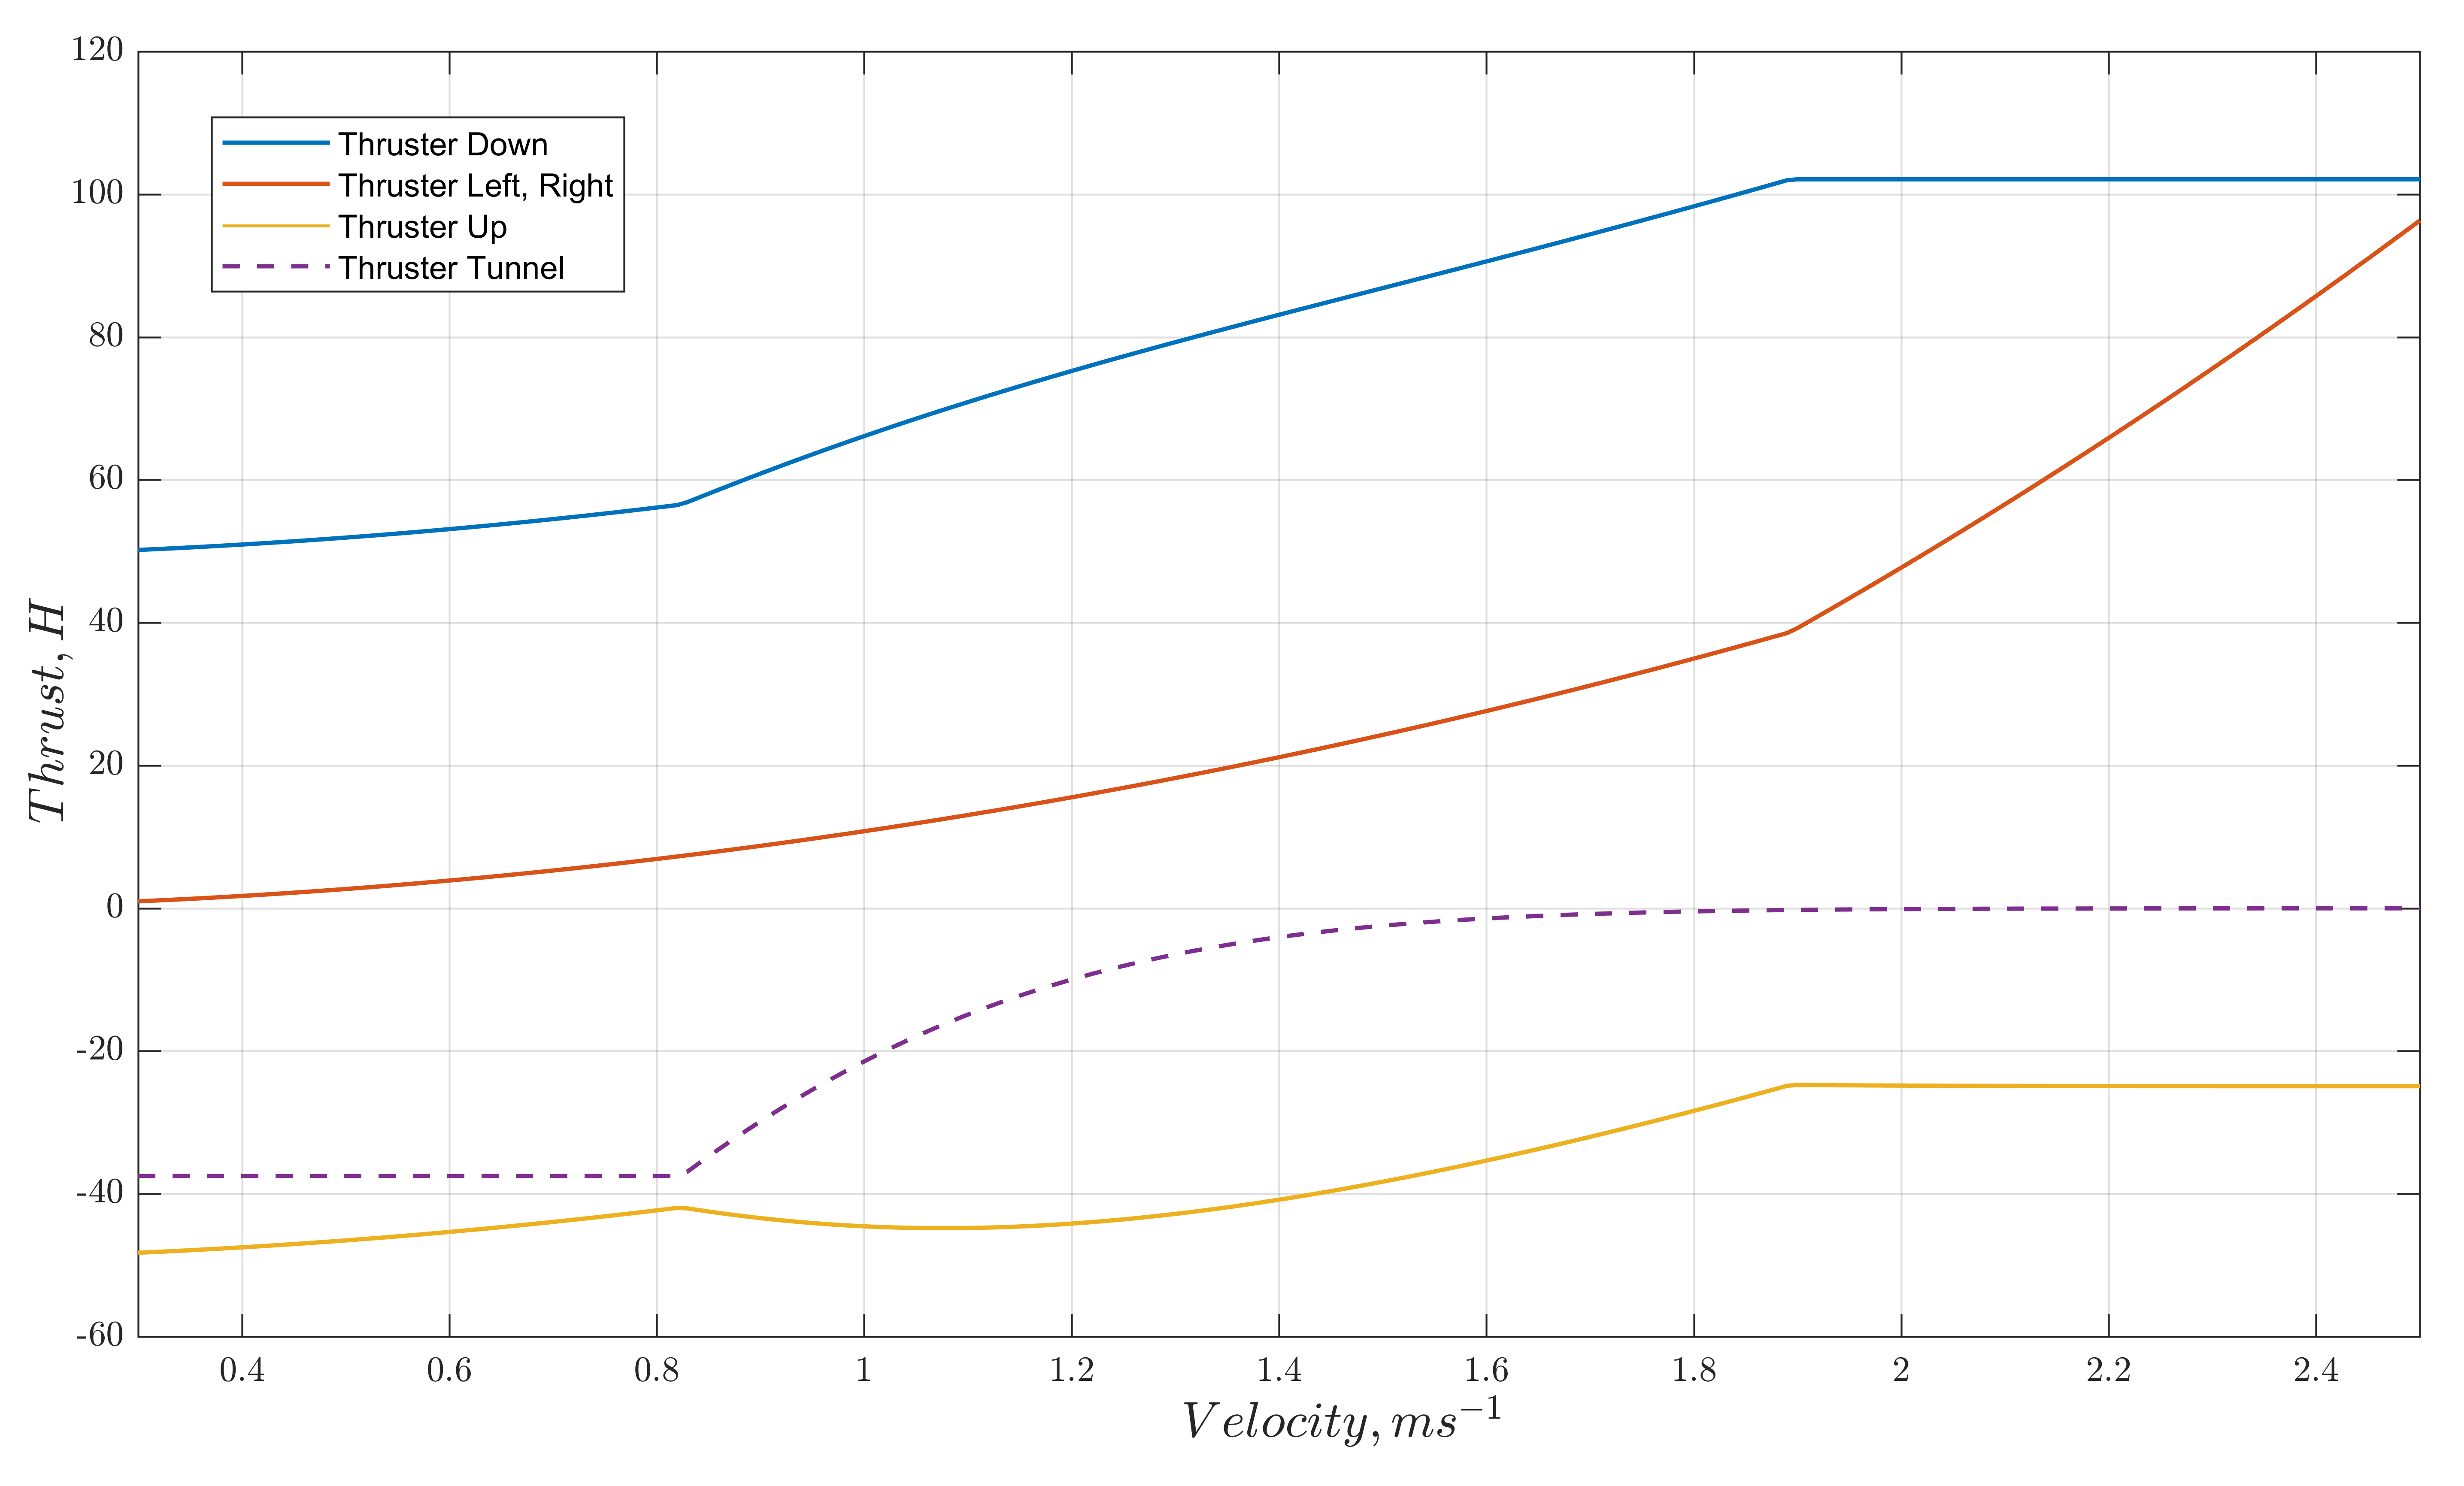
\includegraphics[width=\linewidth]{fig/Allocation_100My.png}
\captionof{figure}{\color{Green} Thrust allocation for different velocities}
\label{plot}
\end{minipage}

\vspace{-2.0cm}
\hspace{37.85cm}
\begin{minipage}[t]{0.48\linewidth}
\color{SaddleBrown}
\bibliographystyle{apalike} % Plain referencing style
\bibliography{sample} % Use the example bibliography file sample.bib
\end{minipage}

\vspace{-14cm}
\color{DarkSlateGray}
\begin{minipage}[t]{0.48\linewidth}
\section*{Conclusions}
To create multi-purpose AUV capable of undertaking both survey-stile missions and low speed interaction requires the more complicated AUV control methods and control allocation.
The quadratic cost optimal approach to constrained control allocation with variable constraints is suggested.
The method takes into account thrust dropping on tunnel thruster on high velocities and reallocation thrust on stern thrusters according to it.
The proposed algorithm was tested on simulation model of real AUV ``MT-2012'' propultion system.
\end{minipage}
\end{document}